% Figure_1.tex -- framework figure (TikZ source), Okabe-Ito colours shared with all data figures. Compile with pdflatex.
% Designed for the full text width (177 mm); lettering is 8 pt sans serif.
\documentclass[10pt,tikz,border=1pt]{standalone}
\usepackage[T1]{fontenc}
\usepackage{amsmath,amssymb}
\usepackage[scaled=0.92]{helvet}
\usetikzlibrary{arrows.meta,fit,calc,backgrounds,positioning}
\definecolor{ink}{HTML}{262626}
\definecolor{joint}{HTML}{0072B2}     % Okabe-Ito blue (J-CBB, uHAC)
\definecolor{indep}{HTML}{D55E00}     % Okabe-Ito vermillion (independent propagation); also dashed outlines
\definecolor{band}{HTML}{F3F3F1}

\begin{document}
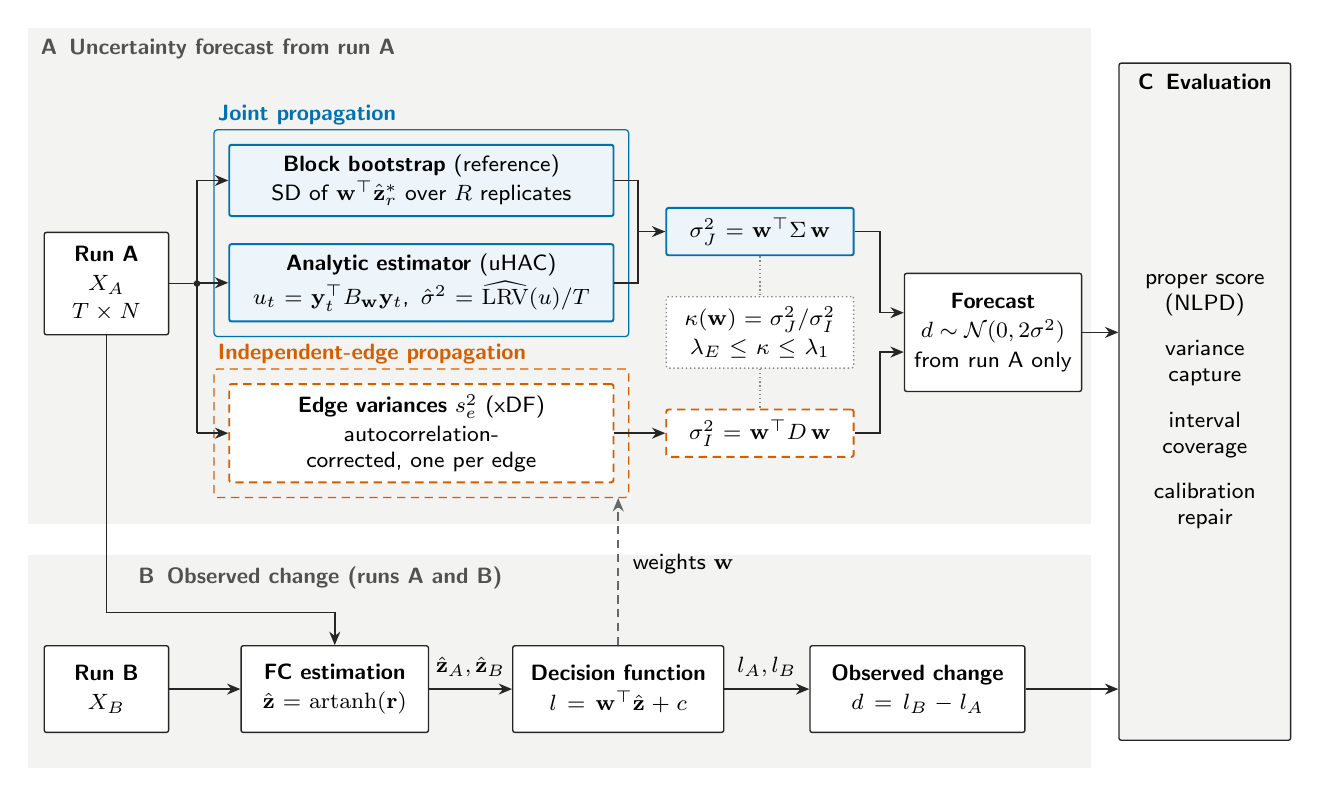
\begin{tikzpicture}[x=1mm, y=1mm,
  font=\sffamily\footnotesize,
  >={Stealth[length=1.7mm,width=1.4mm]},
  box/.style={draw=ink, line width=0.5pt, fill=white, align=center, rounded corners=0.8pt,
              inner xsep=1.4mm, inner ysep=1.3mm},
  jbox/.style={box, draw=joint, line width=0.7pt, fill=joint!7},
  ibox/.style={box, draw=indep, line width=0.7pt, densely dashed, fill=white},
  grp/.style={draw=#1, line width=0.45pt, rounded corners=1.2pt, inner xsep=1.8mm, inner ysep=1.8mm},
  gttl/.style={font=\sffamily\footnotesize\bfseries, inner sep=0.5mm, anchor=south west},
  bttl/.style={font=\sffamily\footnotesize\bfseries, text=ink!80, inner sep=0mm},
  flow/.style={->, draw=ink, line width=0.55pt},
  line/.style={draw=ink, line width=0.55pt}]

% ---------------------------------------------------------------- bands
\begin{scope}[on background layer]
  \fill[band] (-1,30) rectangle (134,93);
  \fill[band] (-1,-1) rectangle (134,26);
\end{scope}
\node[bttl, anchor=north west] at (0.6,91.6) {A\enspace Uncertainty forecast from run A};
\node[bttl, anchor=north west] at (13,24.6) {B\enspace Observed change (runs A and B)};

% ---------------------------------------------------------------- inputs
\node[box, text width=13mm, minimum height=13mm] (xa) at (9,60.5) {\textbf{Run A}\\[0.4mm]$X_A$\\[0.2mm]$T\times N$};
\node[box, text width=13mm, minimum height=11mm] (xb) at (9,9) {\textbf{Run B}\\[0.4mm]$X_B$};

% ---------------------------------------------------------------- propagation (band A)
\node[jbox, text width=46mm] (cbb) at (49,73.6)
  {\textbf{Block bootstrap} (reference)\\[0.3mm] SD of $\mathbf w^{\top}\hat{\mathbf z}^{*}_r$ over $R$ replicates};
\node[jbox, text width=46mm] (uhac) at (49,60.6)
  {\textbf{Analytic estimator} (uHAC)\\[0.3mm] $u_t=\mathbf y_t^{\top}B_{\mathbf w}\mathbf y_t$,\enspace $\hat\sigma^2=\widehat{\mathrm{LRV}}(u)/T$};
\node[ibox, text width=46mm] (xdf) at (49,41.5)
  {\textbf{Edge variances} $s_e^2$ (xDF)\\[0.3mm] autocorrelation-corrected, one per edge};

\node[grp=joint, fit=(cbb)(uhac)] (jg) {};
\node[grp=indep, densely dashed, fit=(xdf)] (ig) {};
\node[gttl, text=joint] (jt) at (jg.north west) {Joint propagation};
\node[gttl, text=indep] (it) at (ig.north west) {Independent-edge propagation};

\node[jbox, text width=21mm] (sj) at (92,67.1) {$\sigma_J^2=\mathbf w^{\top}\Sigma\,\mathbf w$};
\node[ibox, text width=21mm] (si) at (92,41.5) {$\sigma_I^2=\mathbf w^{\top}D\,\mathbf w$};
\node[box, draw=ink!55, densely dotted, text width=21mm] (kap) at (92,54.3)
  {$\kappa(\mathbf w)=\sigma_J^2/\sigma_I^2$\\[0.3mm]$\lambda_E\le\kappa\le\lambda_1$};
\draw[draw=ink!55, densely dotted, line width=0.5pt] (sj.south) -- (kap.north) (kap.south) -- (si.north);

\node[box, text width=20.5mm, inner xsep=1mm, minimum height=15mm] (fc) at (121.6,54.3)
  {\textbf{Forecast}\\[0.4mm] \mbox{$d\sim\mathcal N(0,2\sigma^2)$}\\[0.4mm] from run A only};

% ---------------------------------------------------------------- observation (band B)
\node[box, text width=21mm, minimum height=11mm] (fz) at (38,9) {\textbf{FC estimation}\\[0.4mm]$\hat{\mathbf z}=\operatorname{artanh}(\mathbf r)$};
\node[box, text width=24mm, minimum height=11mm] (dec) at (74,9) {\textbf{Decision function}\\[0.4mm]$l=\mathbf w^{\top}\hat{\mathbf z}+c$};
\node[box, text width=24.5mm, minimum height=11mm] (obs) at (112,9) {\textbf{Observed change}\\[0.4mm]$d=l_B-l_A$};

% ---------------------------------------------------------------- evaluation
\node[box, fill=band, text width=19mm, minimum height=86mm] (ev) at (148.5,45.5) {};
\node[anchor=north, align=center, text width=19mm] at (ev.north) {\\[-1.2mm]\textbf{C\enspace Evaluation}};
\node[align=center, text width=19mm] at (148.5,45.5)
  {proper score\\(NLPD)\\[2.4mm] variance\\capture\\[2.4mm] interval\\coverage\\[2.4mm] calibration\\repair};

% ---------------------------------------------------------------- flows
\coordinate (bus) at (20.5,60.5);
\draw[line] (xa.east) -- (bus);
\draw[line] (bus |- cbb.west) -- (bus |- xdf.west);
\draw[flow] (bus |- cbb.west) -- (cbb.west);
\draw[flow] (bus |- uhac.west) -- (uhac.west);
\draw[flow] (bus |- xdf.west) -- (xdf.west);
\fill[ink] (bus) circle (0.42);

\draw[flow] (cbb.east) -- ++(3,0) |- (sj.west);
\draw[line] (uhac.east) -- ++(3,0) |- (sj.west);
\draw[flow] (xdf.east) -- (si.west);
\draw[flow] (sj.east) -- ++(3.2,0) |- ([yshift=2.5mm]fc.west);
\draw[flow] (si.east) -- ++(3.2,0) |- ([yshift=-2.5mm]fc.west);
\draw[flow] (fc.east) -- (fc.east -| ev.west);

\draw[flow] (xa.south) -- ++(0,-35.2) -| (fz.north);
\draw[flow] (xb.east) -- (fz.west);
\draw[flow] (fz.east) -- node[above=0.3mm] {$\hat{\mathbf z}_A,\hat{\mathbf z}_B$} (dec.west);
\draw[flow] (dec.east) -- node[above=0.3mm] {$l_A,l_B$} (obs.west);
\draw[flow] (obs.east) -- (obs.east -| ev.west);

\draw[flow, draw=ink!70, densely dashed] (dec.north) -- node[right=0.6mm, pos=0.55] {weights $\mathbf w$} (dec.north |- ig.south);
\end{tikzpicture}
\end{document}
